\subsection{Systolic Convolution}
Convolution, though it may not seem intuitive, is just a special case of matrix multiplication.  However, the structure of the equivalent matrix is of special structure (Toeplitz) and is usually sparse, which allows for more efficient implementations than regular matrix multiplication.  For instance, an FIR filter can be realized with the direct form, shown in figure \ref{fig:df1}

\begin{figure}[H]
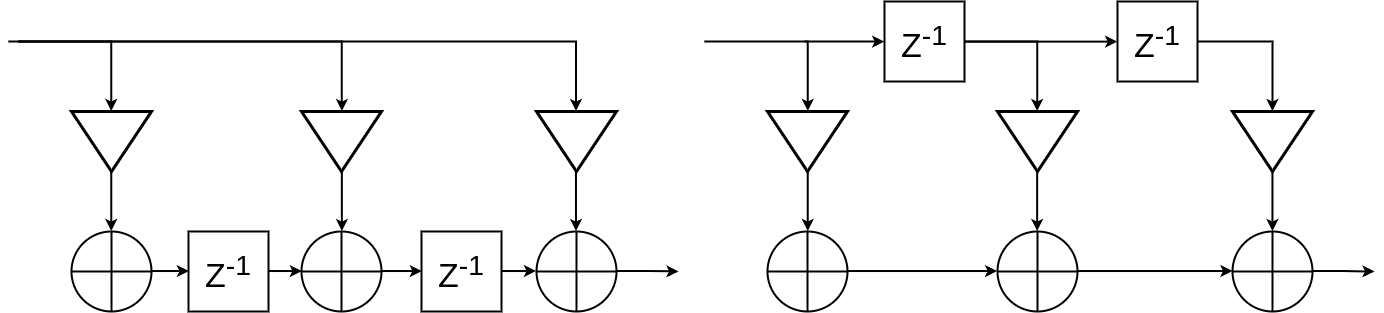
\includegraphics[width=\textwidth]{fir.png}
\caption{Direct Form Transposed (left) and Direct Form (right)}
\label{fig:df1}
\centering
\end{figure}

However, it is clear that if this is actually implemented in hardware, the critical path consists of one multiply and $N$ adders, where $N$ is the length of the filter.  One simple modification, using an adder tree as opposed to an adder chain, would reduce the the critical path to one multiply and $\log_2N$ adders.  However, the direct form transposed, also shown in figure \ref{fig:df1} has a critical path consisting of one multiply and one add, no matter the size of the filter.

Now, each of the multiplies pictured theoretically do not change during the operation of the neural net, so we considered using multiplierless multipliers combined with canonic signed digit represntation for efficient multiplication and filtering.  However, 256 8-tap filters are required for the first convolution stage, meaning we need 2048 multiplies.  However we only have $53,200$ LUTS, and each multiplierless multiplier would require at least 50 LUTS making the design infeasible.  Instead we again turn to time domain multiplexing of the hardware.

Using Xilinx's FIR filter IP core and a controller of our own design, we implemented a component which given a fixed size of data sequentially processes it through each available filter.  This was accomplished by implementing a hybrid queue/circular queue.  First the queue is loaded with samples until full, then whenever a sample is popped from the queue, is broadcast to both the filter and the input of the queue.  This allows the data to repeat for arbitrarily long and so it can be fed through each filter.  The circular queue is a common design pattern in our project since neural nets often have large data parallelism in the form of multiple instruction single data (MISD)

  In the first stage of the neural net, the in-phase and quadrature components of the data are independently filtered with 128 sets of coefficients and then added together.  In order to accomplish this, we instantiated two of the afforementioned components and simply added the result.  We wrote a Python script which verified that the results were correct within error due to fininte precision rounding.
